\section*{Linear Algebra - A Mathematical Background}
A mind-map summarising the key concept of this chapter and their relationship:
\begin{figure}[htbp]
    \centering
    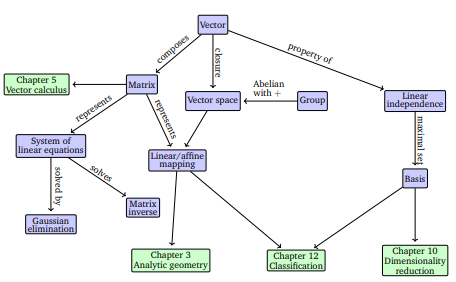
\includegraphics[width= 12cm]{Mathematical Background/mind-map.png}
\end{figure}

\subsection*{Systems of Linear Equations}
Systems of linear equations play a central part of linear algebra. Many problems can be formulated as systems of linear equations, and linear algebra gives us the tools for solving them.\\
In general, for a real-valued system of linear equations we obtain either no, exactly one, or infinitely many solutions. We can introduce a useful compact notation for systems of linear equations ($SLE$) collecting the coefficients $a_{ij}$ into vectors and collect the vectors into matrices.
\begin{align}
    \begin{bmatrix}
        a_{11}\\
        \vdots\\
        a_{m1}
    \end{bmatrix} x_1
    + \begin{bmatrix}
        a_{12}\\
        \vdots\\
        a_{m2}
    \end{bmatrix} x_2
    +\cdots&+
    \begin{bmatrix}
        a_{1n}\\
        \vdots\\
        a_{mn}
    \end{bmatrix} x_n
    = \begin{bmatrix}
        b_{1}\\
        \vdots\\
        b_{m}
    \end{bmatrix}
\end{align}
\begin{align}
    \Longleftrightarrow
    \begin{bmatrix}
        a_{11}& \cdots & a_{1n}\\
        \vdots& & \vdots\\
        a_{m1}& \cdots & a_{mn}
    \end{bmatrix}
    \begin{bmatrix}
        x_{1}\\
        \vdots\\
        x_{m}
    \end{bmatrix}
    &= \begin{bmatrix}
        b_{1}\\
        \vdots\\
        b_{m}
    \end{bmatrix}
\end{align}
\begin{definition}[Homogeneous SLE]
    A system of linear equations is defined as homogeneous if $\vec{b} = \vec{0}$
\end{definition}
%%%%%%%%%%%%%%%%%%%%%%%%%%%%%%%%%%%%%%%%%%
\subsection*{Matrices}
Matrices play a central role in linear algebra and other than to compactly represent $SLE$s they can be used to represent linear functions (linear mappings).

\begin{definition}[Matrix]
    With $m,n \in \mathbb{N}$ a real-valued $(m,n)$ matrix \textbf{A} is an $m\cdot n$-tuple of elements $a_{ij}, i=1,\ldots,n, j=1,\ldots,n$ which is ordere according to a rectangular scheme consisting of $m$ rows and $n$ columns:
\end{definition}
\begin{align}
    \mathbf{A} =
    \begin{bmatrix}
        a_{11} & a_{12} & \cdots & a_{1n}\\
        a_{21} & a_{22} & \cdots & a_{2n}\\
        \vdots & \vdots &  & \vdots\\
        a_{m1} & a_{m2} & \cdots & a_{mn}
    \end{bmatrix}, \quad a_{ij} \in \mathbb{R}
\end{align}
By convention $(1,n)$-matrices are called rows and $(m,1)$-matrices are called columns. These special matrices are also called row/column vectors.\\
For matrices $\mathbf{A} \in \mathbb{R}^{m\times n},\mathbf{B} \in \mathbb{R}^{n\times k}$, the elements $c_{ij}$ of the product $\mathbf{C} = \mathbf{AB} \in \mathbb{R}^{m\times k}$ are computed as follows:
\[
    c_{ij}= \sum_{l=1}^{n}{a_{il}b_{lj}}, \quad i=1,\ldots,m \quad j=1, \ldots, k  
\]
This means that the elements of the $i$th-row of \textbf{A} are multiplied with the elements of the $j$th-column of \textbf{B} and then summed together.
\begin{definition}[Identity Matrix]
    In $\mathbb{R}^{n\times n}$, we define the identity matrix as the $n \times n$ matrix containing 1 on the diagonal and 0 everywhere else. 
\end{definition}
With the understanding of matrix multiplication, matrix addition and the identity matrix we can take a look at some properties of matrices:
\begin{description}
    \item[Associativiy:]\[
        \forall \mathbf{A} \in \mathbb{R}^{m\times n}, \mathbf{B} \in \mathbb{R}^{n\times p}, \mathbf{C} \in \mathbb{R}^{p\times q}: (\mathbf{AB})\mathbf{C} = \mathbf{A}(\mathbf{BC})
    \]
    \item[Distributivity] \begin{align}
        \forall \mathbf{A,B} \in \mathbb{R}^{m\times n}, \mathbf{C,D} \in \mathbb{R}^{n\times p}: &(\mathbf{A}+\mathbf{B})\mathbf{C}= \mathbf{AC}+\mathbf{BC} \\ 
        &\mathbf{A}(\mathbf{C}+\mathbf{D})= \mathbf{AC}+\mathbf{AD}
    \end{align}
\end{description}
\begin{definition}[Inverse]
    Consider a square matrix $\mathbf{A} \in \mathbb{R}^{n\times n}$. Let matrix $\mathbf{B} \in \mathbb{R}^{n\times n}$ have the property that $\mathbf{AB} = \mathbf{I}_n = \mathbf{BA}$. $\mathbf{B}$ is called the inverse of $\mathbf{A}$ and denoted by $\mathbf{A}^{-1}$
\end{definition}
Unfortunately not every matrix possesses and inverse. If this inverse does exist the matrix is called regular/invertible/nonsingular; otherwise it's called singular/noninvertible.
\begin{definition}[Transpose]
    For $\mathbf{A} \in \mathbb{R}^{m\times n}$ the matrix $\mathbf{B} \in \mathbb{R}^{n\times m}$ with $b_{ij}= a_{ji}$ is called the transpose of $\mathbf{A}$. We write it as $\mathbf{B} = \mathbf{A}^T$
\end{definition}
\begin{definition}[Symmetric Matrix]
    A matrix $\mathbf{A} \in \mathbb{R}^{n\times n}$ is symmetric if $\mathbf{A} = \mathbf{A}^T$
\end{definition}
\subsubsection*{Compact Representations of SLE}
If we consider a system of linear equations and use the rules for matrix multiplication, we can write this equation system in a more compact form:
\[
    \begin{bmatrix}
        2 & 3 & 5 \\
        4 & -2 & -7 \\
        9 & 5 & -3
    \end{bmatrix}
    \begin{bmatrix}
        x_1 \\
        x_2\\
        x_3
    \end{bmatrix}
    =
    \begin{bmatrix}
        1 \\
        8\\
        2
    \end{bmatrix}
\]
Generally a system of linear equations can be compactly represented in their matrix form as $\mathbf{A}x=b$.\\
\begin{definition}[Row-Echelon Form REF]
    A matrix is in row-echelon form if:
    \begin{itemize}
        \item All rows that contain only zeros are at the bottom of the matrix; correspondigly, all rows that contain at least one nonzero element are on top of rows that contain only zeros.
        \item Looking at nonzero rows only, the first nonzero number from the left (also called the pivot or the leading coefficient) is always strictly to the right of the pivot of the row above it
    \end{itemize}
\end{definition}
\begin{remark}[Reduced Row-Echelon Form] An equation system is in reduced row-echelon form (also row-reduces echelon form or row canonical form) if:
    \begin{itemize}
        \item It is in row-echelon form
        \item Every pivot is 1
        \item The pivot is the only nonzero entry in its column
    \end{itemize}
\end{remark}

\subsection*{Vector Spaces}
So far we have seen that systems of linear equations can be compactly represented using matrix-vector notation. In the following chapter we will have a closer look at vector spaces, i.e., a structured space in which vectors live.
\subsubsection*{Groups}
We are ready to formalize the characteristics of vectors and scalar multiplication but we need to introduce the concept of a group. A group is a set of elements and an operation defined on these elements that keeps some structure of the set intact.
Groups play an important role in computer science. Besides providing a fundamental framework for operations on sets, they are heavily used in cryptography, coding theory and graphics.
\begin{definition}[Group]
    Consider a set $\mathcal{G}$ and an operation $\otimes: \mathcal{G} \times \mathcal{G} \rightarrow \mathcal{G}$ defined on $\mathcal{G}$. Then $G:=(\mathcal{G},\otimes)$ is called a group if the following hold:
    \begin{enumerate}
        \item Closure of $\mathcal{G}$ under $\otimes: \forall x,y \in \mathcal{G}: x\otimes y \in \mathcal{G}$
        \item Associativiy: $\forall x,y,z \in \mathcal{G}: (x\otimes y) \otimes z = x \otimes(y \otimes z)$
        \item Neutral element: $\exists e \in \mathcal{ G} \forall x \in \mathcal{G} : x\otimes e = x$ and $e \otimes x =x$
        \item Inverse element: $\forall x \in \mathcal{G} \exists y\in \mathcal{G}: x\otimes y = e$ and $y\otimes x = e$, where $e$ is the neutral element. We oftern write $x^{-1}$ to denote the inverse element of x.
    \end{enumerate}
\end{definition}
\begin{remark}[Abelian Group]
    If additionally $\forall x,y \in \mathcal{G}: x\otimes y = y\otimes x$, then $G = (\mathcal{G,\otimes})$ is an Abelian group (commutative).
\end{remark}
\subsubsection*{Vector Spaces}
We will now consider an extension of the definition of group that in addition to an inner operation $+$ also contain an outer operation $\cdot$, the multiplication of a vector $x\in \mathcal{G}$ by a scalar $\lambda \in \mathbb{R}$.
\begin{definition}[Vector space]
    A real-valued vector space $V = (\mathcal{V}, +, \cdot)$ is a set $\mathcal{V}$ with two operations
    \begin{align*}
        + : \mathcal{V} \times \mathcal{V} \rightarrow \mathcal{V}\\
        \cdot : \mathbb{R}  \times \mathcal{V} \rightarrow \mathcal{V}
    \end{align*}
    where
    \begin{enumerate}
        \item $(\mathcal{V},+)$ is an Abelian group
        \item Distributivity
        \item Associativiy (w.r.t. the outer operation)
        \item Neutral element (w.r.t. the outer operation)
    \end{enumerate}
\end{definition}
The elements $x \in V$ are called vectors.
\begin{remark}
    A "vector multiplication" $\mathbf{ab}, a,b \in \mathbb{R}^n$ is not defined. We could use the matrix multiplication as previously defined however the dimensions of the vectors do not match. Only the following multiplication for vectors are defined: $\mathbf{ab}^T \in \mathbb{R}^{n\times n}$ (outer product), $\mathbf{a^Tb}\in \mathbb{R}$ (inner/scalar/dot product)
\end{remark}

%%%%%%%%%%%%%%%%%%%%%%%%%%%%%%%%%%%%%%%%%%%%%%%%%%%%%%%%%%%%%%%%%
\subsubsection*{Vector Subspaces}
Intuitively, vector subspaces are sets contained in the original vector space with the property that when we perform space operations on elements within this subspace, we will never leave it. In this sense they are "closed". We will see how we can use vector subspaces to perform dimensionality reduction.
\begin{definition}[Vector subspace]
    Let $V = (\mathcal{V}, +, \cdot)$ be a vector space and $\mathcal{U} \subseteq \mathcal{V}, \mathcal{U} \neq \emptyset$. Then $U = (\mathcal{U},+,\cdot)$ is called vector subspace of V (or linear subspace) if $U$ is a vector space with the vector space operations + and $\cdot$ restricted to $\mathcal{U} \times \mathcal{U}$ and $\mathbb{R} \times \mathcal{U}$. We write $U \subseteq V$ to denote a subspace $U$ of $V$.
\end{definition}
If $U$ is a vector subspace of $V$ it naturally inherits many of its properties but to determine whether $(\mathcal{U}, +, \cdot)$ is a subspace of V we still need to show
\begin{enumerate}
    \item $\mathcal{U} \neq \emptyset$, in particular $\vec{0} \in \mathcal{U}$
    \item Closure of $U$:
    \begin{enumerate}
        \item W.r.t. to the outer operation: $\forall \lambda \in \mathbb{R} \forall x \in \mathcal{U}: \lambda x \in \mathcal{U}$
        \item W.r.t. to the outer operation: $\forall x,y \in \mathcal{U}: x + y \in \mathcal{U}$
    \end{enumerate}
\end{enumerate}
Example:
\begin{figure}[htbp]
    \centering
    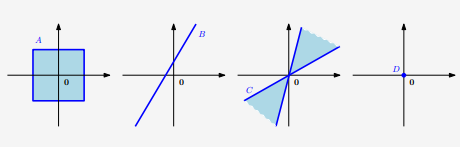
\includegraphics[width=10cm]{Mathematical Background/example-subspace-recognition.png}
\end{figure}
Only example D in the followin figureì is a subspace of $R^2$ (with the inner/outer operations). In A and C the closure property is violated, meanwhile B does not contain $\vec{0}$.
\begin{remark}
    Every subspace $U \subseteq (R^n, + ,\cdot)$ is the solution space of a homogeneous SLE $\mathbf{A}\vec{x} = \vec{0}$ for $\vec{x} \in R^n$
\end{remark}
\subsubsection*{Linear Indipendence}
In the following subsection we will take a closer look at what we can do with vectors. In particular, we can add vectors together and multiply them with scalars. The closure property guarantees that we end up with another vector in the same vector space. It is possible, we will see, to find a set of vectors with which we can represent every vector in the vector space by adding them together and scaling them. This set of vectors is a basis. Before we can explore further these concept we need to define linear combinations and linear indipendence.

\begin{definition}[Linear combination]
    Consider a vector space $V$ and a finite number of vectors $x_1,\ldots, x_k \in V$. Then, every $v \in V$ of the form
    \[
        v = \lambda_1x_1 + \cdots + \lambda_kx_k = \sum_{i=1}^{k}{\lambda_ix_i} \in V
    \] 
    with $\lambda_1,\ldots,\lambda_k \in \mathbb{R}$ is a linear combination of the vectors $x_1,\ldots, x_k$
\end{definition}
The $\vec{0}$ can always be written as the linear combination of $k$ vectors, only some of them are non-trivial. In the following we are interested in non-trivial linear combinations that represent $\vec{0}$, that is, where not all $\lambda_i$ are 0.
\begin{definition}[Linear (In)dependence]
    Let us consider a vector space $V$ with $k \in \mathbb{N}$ and $x_i, \ldots, x_k \in V$. If there is a non-trivial linear combination, such that $\vec{0} = \sum_{i=1}^{k}{\lambda_ix_i}$ with at least one $\lambda_i \neq 0$, the vectors $x_1,\ldots, x_k$ are linearly dependent. If only the trivial solution exists the vectors $x_1, \ldots, x_k$ are linearly independent.
\end{definition}
Intuitively a set of linearly independent vectors consists of vectors that have no redundancy. If we remove any of those vectors from the set, we will lose something.
\begin{remark}
    Consider a vector space $V$ with $k$ linearly independent vectors $b_1,\ldots,b_k$ and $m$ linear combinations
    \[
        x_j = \sum_{i=1}^{k}{\lambda_i1b_i}, \quad j= 1,\ldots, m
    \]
    Defining $\mathbf{B} = [b_1,\ldots,b_k]$ as the matrix whose columns are the linearly independent vectors $b_1,\ldots,b_k$, we can write in a more compact form
    \[
        x_j = \mathbf{B}\lambda_j, \quad \lambda_j = \begin{bmatrix}
            \lambda_{1j}\\ \vdots \\ \lambda_{kj}
        \end{bmatrix}, \quad j = 1,\ldots, m
    \]
\end{remark}
A set of vectors are linearly independent if and only if no-one of the vectors can be obtained as a linear combination of the others.\\
%%%%%%%%%%%%%%%%%%%%%%%%%%%%%%%%%%%%%%%%%%%%%%%%%%%%%
\subsection*{Basis and Rank}
In a vector space $V$, we are particularly interested in sets of vectors $\mathcal{A}$ that possess the property that any vector $v \in V$ can be obtained by a linear combination of the vectors in $\mathcal{A}$.
\subsubsection*{Generating Set and Basis}
\begin{definition}[Generating set and Span]
    Consider a vector space $V = (\mathcal{V},+,\cdot)$ and set of vectors $\mathcal{A} = {x_1,\ldots,x_k} \subseteq \mathcal{V}$. If every vector $v \in \mathcal{V}$ can be expressed as a linear combination of $x_1, \ldots, x_k$, $\mathcal{A}$ is called a generating set of V. The set of all linear combinations of vectors in $A$ is called the span of $\mathcal{A}$. If $\mathcal{A}$ spans the vector space $V$, we write $V = span[\mathcal{A}]$ or $V = span[x_1,\ldots,x_k]$
\end{definition}
\begin{definition}[Basis]
    Consider a vector space $V = (\mathcal{V},+,\cdot)$ and $\mathcal{A} \subseteq \mathcal{V}$. A generating set $\mathcal{A}$ of $V$ is called minimal if there exists no smaller set $\tilde{\mathcal{A}}\subsetneq \mathcal{A} \subseteq \mathcal{V}$ that spans $V$. Every linearly independent generating set of $V$ is minimal and is called a basis of $V$
\end{definition}
In our study we will only consider finite-dimensional vector spaces $V$. In this case, the dimension of V is the number of basis vectors of $V$, and we write $dim(V)$. If $U\subseteq V$ is a subspace of $V$, then $dim(U) \leq dim(V)$ and $dim(U) = dim(V)$ if and only if $U=V$. Intuitively, the dimension of a vector space can be thought of as the number of independent directions in this vector space. However, it is important to notice that this is not necessarily the number of elements in a basis vector but it is the number of basis vectors.
\begin{remark}
    A basis of a subspace $U = span[x_1,\ldots,x_m] \subseteq R^n$ can be found by executing the followin steps:
    \begin{enumerate}
        \item Write the spanning vectors as columns of a matrix $\mathbf{A}$
        \item Determine the row-echelon form of $\mathbf{A}$
        \item The spanning vectors associtated with the pivot columns are a basis of $U$
    \end{enumerate}
\end{remark}

\subsubsection*{Rank}
The number of linearly independent columns of a matrix $\mathbf{A} \in \mathbb{R}^{m\times n}$ equals the number of linearly independent rows and is called the rank of $\mathbf{A}$ and is denoted by $rk(\mathbf{A})$.\\
The columns of $\mathbf{A} \in \mathbb{R}^{m\times n}$ span a subspace $U \subseteq \mathbb{R}^m$ with $dim(U) = rk(\mathbf{A})$. Later we will call this subspace the image or range.\\
For all $\mathbf{A} \in \mathbb{R}^{n\times n}$ it holds that $\mathbf{A}$ is regular (invertible) if and only if $rk(\mathbf{A}) = n$\\
A matrix $\mathbf{A} \in R^{m\times n}$ has full rank if its rank equals the largest possible rank for a matrix of the same dimensions. This means that the rank of
a full-rank matrix is the lesser of the number of rows and columns, i.e.,
$rk(A) = min(m, n)$. A matrix is said to be rank deficient if it does not
have full rank.

\subsection*{Linear Mappings}
In this section we will study mappings on vector spaces that preserve their structure, which will allow us to define the concept of a coordinate. In the beginning of the chapter we said that vectors are objects that can be added together and multiplied by a scalar, and the resulting object is still a vector. We wish to preserve this property when applying the mapping. Consider two real vector spaces $V,W$, a mapping $\Phi : V \longrightarrow W $ preserves the structure of the vector space if
\begin{align}
    \Phi(\vec{x}+\vec{y}) &= \Phi(\vec{x})+\Phi(\vec{y})\\
    \Phi(\lambda \vec{x}) &= \lambda \Phi(\vec{x})
\end{align}
for all $x,y \in V$ and $\lambda \in \mathbb{R}$. We can summarize this in the following definition.
\begin{definition}[Linear Mapping]
    For vector spaces $V,W$, a mapping $\Phi : V \longrightarrow W$ is called a linear mapping (or vector space homomorphism/linear transformation) if
    \[
        \forall x,y \in V \; \forall \lambda,\psi \in \mathbb{R}: \Phi(\lambda x+\psi y) = \lambda\Phi(x)+\psi \Phi(y)
    \]
\end{definition}
It turns out that we can represent linear mappings as matrices. Recall that we can also collect a set of vectors as columns of a matrix. When working with matrices, we have to keep in mind what the matrix represents: a linear mapping or a collection of vectors.
\begin{definition}[Injective, Surjective and Bijective mappings]
    Consider a mapping $\Phi : \mathcal{V} \longrightarrow \mathcal{W}$ where $\mathcal{V},\mathcal{W}$ can be arbitrary sets. Then $\Phi$ is called
    \begin{description}
        \item[Injective]: if $\forall x,y \in \mathcal{V}: \Phi(x) = \Phi(y) \Longrightarrow x = y$
        \item[Surjective]:if $\Phi(\mathcal{V}) = \mathcal{W}$
        \item[Bijective]: if $\Phi$ is both injective and surjective.  
    \end{description}
\end{definition}
\begin{theorem}
    Two finite-dimensional vector spaces $V$ and $W$ are isomorphic if and only if $dim(V) = dim(W)$
\end{theorem}
\subsubsection*{Matrix Representation of Linear Mappings}
From the theorem just presented we can derive that any n-dimensional vector space is isomorphic to $R^n$. We can consider a basis ${b_1,\ldots,b_n}$ of an n-dimensional vector space $V$. In the following subsection the order of the basis vectors will be important, therefore, we write
\[
    B = (b_1,\ldots,b_n)
\]
and we call this n-tuple an ordered basis of V.
\begin{remark}[Notation]
    In order to keep things straight we summarise some parts of the notation here. $B = (b_1,\ldots,b_n)$ is an ordered basis, $\mathcal{B} = \{b_1,\ldots,b_n\}$ is an (unordered) basis, and $\mathbf{B} = [b_1,\ldots,b_n]$ is a matrix whose columns are the vectors $b_1,\ldots, b_n$
\end{remark}
\begin{definition}[Coordinates]
    Consider a vector space $V$ and an ordere basis $B = (b_1,\ldots,b_n)$ of $V$. For any $x \in V$ we obtain a unique representation (linear combination) of x with respect to $B$
    \[
        x = \alpha_1b_1+\ldots+\alpha_nb_n  
    \]
    Then $\alpha_1,\ldots,\alpha_n$ are the coordinates of x with respect to $B$, and the vector
    \[
        \vec{\alpha} =
        \begin{bmatrix}
            \alpha_1\\
            \vdots\\
            \alpha_n
        \end{bmatrix} \in \mathbb{R}^n
    \]
    is the coordinate vector or the coordinate representation of x with respect to the ordered basis $B$.
\end{definition}
\begin{definition}[Transformation Matrix]
    Consider vector spaces $V,W$ with corrsponding (ordered) basis $B = (b_1,\ldots,b_n)$ and $C = (c_1,\ldots,c_m)$. Moreover, we consider a linear mapping $\Phi : V \longrightarrow W$. For $j \in {1,\ldots,n}$,
    \[
        \Phi(b_j) = \alpha_{1j}c_1+ \cdots + \alpha_{mj}c_m = \sum_{i=1}^{m}{a_{ij}c_i}  
    \]
    is the unique representation of $\Phi(b_j)$ with respect to $C$. Then, we call the $m\times n$ matrix $\mathbf{A}_{\Phi}$, whose elements are given by
        \[
            \mathbf{A}_{\Phi}(i,j) = \alpha_{i,j}
        \]
    the transformation matrix of $\Phi$ (with respect to the ordered bases $B$ of $V$ and $C$ of $W$)
\end{definition}
Consider (finite-dimensional) vector spaces $V,W$ with ordered bases $B,C$ and a linear mapping $\Phi: V \longrightarrow W $with transformation matrix $\mathbf{A}_{\Phi}$. If $\hat{x}$ is the coordinate vector of $x \in V$ with respect to $B$ and $\hat{y}$ the coordinate vector of $y = \Phi(x) \in W$ with respect to $C$, then
\[
    \hat{y} = \mathbf{A}_{\Phi}\hat{x}    
\]
This means that the transformation matrix can be used to map coordinates with respect to an ordered basis in $V$ to coordinates with respect to an ordered basis in $W$
\begin{figure}[htbp]
    \centering
    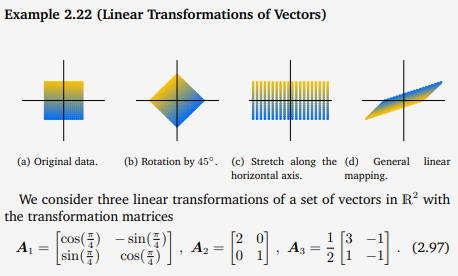
\includegraphics[width=12cm]{Mathematical Background/example-transformation-matrix-application.png}
\end{figure}\\
\textbf{Questions:}\\
Where do the coefficients $\alpha_{ij}$ of the transformation matrix come from? Can we follow an example of calculating the transformation of one of the vectors from the image?
\subsubsection*{Basis Change}
\subsubsection*{Image and Kernel}
Dimentionality reduction:
Image or kernel\\
for $\Phi : V \rightarrow W$ we define the kernel/null space:
$$ker(\Phi) = \Phi^{-1}(0_w) = {v \in V, \Phi(v) = 0_w}$$
$$Im(\Phi) = $$